\documentclass{sig-alternate-05-2015}
%\documentclass{llncs}
\usepackage{makeidx}
\usepackage{tabularx,colortbl}
\usepackage[dvipsnames]{xcolor}
\usepackage{flushend}
\usepackage{cite}
\usepackage{amsmath}
%\usepackage{amsthm}
\usepackage{amssymb}
\usepackage{epsfig}
\usepackage{stmaryrd}
\usepackage{url}
\usepackage{multirow}
\usepackage{latexsym}
\usepackage{graphics}
\usepackage{graphicx}
\usepackage{enumitem}
\usepackage{comment}
\usepackage{longtable}
\usepackage{supertabular}
\usepackage{times}
\usepackage{listings}
\usepackage{subfigure}
\usepackage{color}
\usepackage{balance}
\usepackage{xspace}
\usepackage[ruled, vlined, linesnumbered]{algorithm2e}
\usepackage[autostyle]{csquotes}



%\theoremstyle{Definition}
%\newtheorem{definition}{Definition}
%%%
%\theoremstyle{Theorem}
%\newtheorem{theorem}{Theorem}


%\newcommand{\definition}{\noindent \textbf{Definition} \citation{}}
%\newcommand{\theorem}{\noindent \textbf{Theorem} \citation{}}
%\newcommand{\lemma}{\noindent \textbf{Lemma} \citation{}}

%\newdef{lemma}{Lemma}
%\newdef{definition}{Definition}
%\newdef{theorem}{Theorem}
%\newdef{corollary}{Corollary}
%\newdef{note}{Note}
%\newdef{axiom}{Axiom}
\newcommand{\mkeyword}[1]{\mbox{\texttt{#1}}}
\DeclareMathOperator{\kuop}{uop}
\DeclareMathOperator{\kbop}{bop}
\DeclareMathOperator{\kite}{ite}
\DeclareMathOperator{\kpre}{pre}
\DeclareMathOperator{\dom}{dom}
\DeclareMathOperator{\ktrue}{true}
\DeclareMathOperator{\kfalse}{false}
\DeclareMathOperator{\kselect}{select}
\DeclareMathOperator{\ran}{range}
\definecolor{mypink}{rgb}{0.858, 0.188, 0.478}
\newcommand{\lbb}{[\![}
\newcommand{\rbb}{]\!]}
\newcommand{\expr}{\phi}
\newcommand{\exprS}{\Phi}
\newcommand{\mike}[1]{\textcolor{red}{#1}}
\newcommand{\janet}[1]{\textcolor{blue}{#1}}
\newcommand{\darren}[1]{\textcolor{green}{#1}}
\newcommand{\danielle}[1]{\textcolor{orange}{#1}}

\sloppypar



\begin{document}
\CopyrightYear{2016}
\setcopyright{acmcopyright}
%\conferenceinfo{FSE'16,}{November 13-19, 2016, Seattle, WA, USA}
%\isbn{978-1-4503-4218-6/16/11}\acmPrice{\$15.00}
%\doi{http://dx.doi.org/10.1145/2950290.2950346}

\definecolor{gold}{rgb}{0.90,.66,0}
\definecolor{dgreen}{rgb}{0,0.6,0}
\newcommand{\stateequiv}{\equiv_{s}}
\newcommand{\traceequiv}{\equiv_{\sigma}}
\newcommand{\ta}{\text{TA}}
\newcommand{\cta}{\text{TA$_{C}$}}
\newcommand{\tta}{\text{TA$_{T}$}}
\newcommand{\ucalg}{\texttt{\small{IVC\_UC}}}
\newcommand{\ucbfalg}{\texttt{\small{IVC\_UCBF}}}
\renewcommand{\abstract}{\noindent {\sc \textbf{\large {Architectural Modeling and Analysis\\for Safety Engineering}}}\\}


% paper title
% can use linebreaks \\ within to get better formatting as desired
\title{Written Preliminary Examination Report}
%\subtitle{[subtitle]
%\titlenote{A full version of this paper is available as
%\textit{Author's Guide to Preparing ACM SIG Proceedings Using
%\LaTeX$2_\epsilon$\ and BibTeX} at
%\texttt{www.acm.org/eaddress.htm}}}
\numberofauthors{1} %  in this sample file, there are a *total*
% of EIGHT authors. SIX appear on the 'first-page' (for formatting
% reasons) and the remaining two appear in the \additionalauthors section.
%
\author{
% You can go ahead and credit any number of authors here,
% e.g. one 'row of three' or two rows (consisting of one row of three
% and a second row of one, two or three).
%
% The command \alignauthor (no curly braces needed) should
% precede each author name, affiliation/snail-mail address and
% e-mail address. Additionally, tag each line of
% affiliation/address with \affaddr, and tag the
% e-mail address with \email.
%
% 1st. author
\alignauthor
Danielle Stewart\\
       \affaddr{Department of Computer Science \& Engineering}\\
       \affaddr{University of Minnesota}\\
       \affaddr{MN, USA}\\
       \email{dkstewar@umn.edu}
       }



\maketitle

\begin{abstract}
This paper describes a new methodology with tool support for model-based safety analysis. It is implemented as a {\em Safety Annex} for the Architecture Analysis and Design Language (AADL). The Safety Annex provides the ability to describe faults and faulty component behaviors in AADL models. In contrast to previous AADL-based approaches, the Safety Annex leverages a formal description of the nominal system behavior to propagate faults in the system. This approach ensures consistency with the rest of the system development process and simplifies the work of safety engineers. The language for describing faults is extensible and allows safety engineers to weave various types of faults into the nominal system model. The Safety Annex supports the injection of faults into component level outputs, and the resulting behavior of the system can be analyzed using model checking through the Assume-Guarantee Reasoning Environment (AGREE).
\end{abstract}

\keywords{Model-based systems engineering; fault analysis; safety engineering}

\section{Introduction}
\label{sec:intro}

%This paper describes a new methodology with tool support for model based safety analysis. It is implemented as a {\em Safety Annex} for the Architecture Analysis and Design Language (AADL). The Safety Annex provides the ability to describe faults and faulty component behaviors in AADL models. In contrast to previous AADL-based approaches, the Safety Annex leverages a formal description of the nominal system behavior to propagate faults in the system. This approach ensures consistency with the rest of the system development process and simplifies the work of safety engineers. The language for describing faults is extensible and allows safety engineers to weave various types of faults into the nominal system model. The Safety Annex supports the injection of faults into component level outputs, and the resulting behavior of the system can be analyzed using model checking through the Assume-Guarantee Reasoning Environment (AGREE).

System safety analysis techniques are well-established and are a required activity in the development of safety-critical systems. Model-based systems engineering (MBSE) methods and tools based on formal methods now permit system-level requirements to be specified and analyzed early in the development process~\cite{NFM2012:CoGaMiWhLaLu,CAV2015:BoCiGrMa}. While model-based development methods are widely used in the aerospace industry, they are only recently being applied to system safety analysis.  

%How can we leverage these model-based methods and tools to perform safety analysis based on models of the system architecture and initial functional decomposition? Can these design models be integrated into the safety analysis process to help guarantee accurate and consistent results?
%Seeking solutions to these questions are especially important as the amount of safety-critical hardware and software in various domains has drastically increased due to the demand for greater autonomy, capability, and connectedness.

In this paper, we describe a {\em Safety Annex} for the Architecture Analysis and Design Language (AADL)~\cite{FeilerModelBasedEngineering2012} that provides the ability to reason about faults and faulty component behaviors in AADL models. In the Safety Annex approach, we use formal assume-guarantee contracts to define the nominal behavior of system components. The nominal model is then verified using the Assume Guarantee Reasoning Environment (AGREE)~\cite{NFM2012:CoGaMiWhLaLu}. The Safety Annex  provides a way to weave faults into the nominal system model and analyze the behavior of the system in the presence of faults. The Safety Annex also provides a library of common fault node definitions that is customizable to the needs of system and safety engineers. Our approach adapts the work of Joshi et. al in
~\cite{Joshi05:Dasc} to the AADL modeling language, and provides a domain specific language for the kinds of analysis performed manually in previous work~\cite{Stewart17:IMBSA}.  %More information on the approach is available in~\cite{Stewart17:IMBSA}, and the tool and relevant documentation can be found at: \small \url{https://github.com/loonwerks/AMASE/}. \normalsize

There are other tools purpose-built for safety analysis, including AltaRica~\cite{PROSVIRNOVA2013127}, smartIFlow~\cite{info8010007} and xSAP~\cite{DBLP:conf/tacas/BittnerBCCGGMMZ16}. These notations are separate from the system development model. Other tools extend existing system models, such as HiP-HOPS~\cite{CHEN201391} and the AADL Error Model Annex, Version 2 (EMV2)~\cite{EMV2}. EMV2 uses enumeration of faults in each component and explicit propagation of faulty behavior to perform safety analysis. The required propagation relationships must be manually added to the system model and can become complex, leading to potential omissions and inconsistencies.

In contrast, the Safety Annex supports model checking and quantitative reasoning by attaching behavioral faults to components and then using the normal behavioral propagation and proof mechanisms built into the AGREE AADL annex. This allows users to reason about the evolution of faults over time, and produce counterexamples demonstrating how component faults lead to system failures. It can serve as the shared model to capture system design and safety-relevant information, and produce both qualitative and quantitative description of the causal relationship between faults/failures and system safety requirements.
%
Thus, the contributions of the Safety Annex and this paper are:
\begin{itemize}
\item Close integration of behavioral fault analysis into an {\em architectural design language} AADL, which allows close connection between system and safety analysis and system generation from the model (unlike AltaRica, smartIFlow, and xSAP),
\item support for {\em behavioral specification of faults} and their {\em implicit propagation} through behavioral relationships in the model, in contrast to existing AADL-based annexes (HiP-HOPS and EMV2),
\item additional support for {\em explicit} propagation of faults to capture binding relationships between hardware and software and logical and physical communications beyond what is supported in xSAP, and
\item guidance on integration into a traditional safety analysis process.
\end{itemize}
%\mike{What are our contributions?}


\section{Model-Based Safety Analysis}

%\mike{Audience should already know about model-based safety analysis.  We want to discuss two ``strands'' of MBSA, one with explicit fault propagation of faults rather than system dynamics, and another based on faults propagating through their effects on dynamics}.

A model-based approach for safety analysis was proposed by Joshi et. al in \cite{Joshi05:Dasc, Joshi05:SafeComp, Joshi07:Hase}.  In this approach, a safety analysis system model (SASM) is the central artifact in the safety analysis process, and traditional safety analysis artifacts, such as fault trees, are automatically generated by tools that analyze the SASM.

The contents and structure of the SASM differ significantly across different conceptions of MBSA.  We can draw distinctions between approaches along several different axes.  The first is whether models and notations are purpose-built for safety analysis (such as AltaRica~\cite{PROSVIRNOVA2013127}, smartIflow~\cite{info8010007} and xSAP~\cite{DBLP:conf/tacas/BittnerBCCGGMMZ16}) vs. those that extend existing system models (ESM) (HiP-HOPS~\cite{CHEN201391}, the AADL error annex\cite{SAEAS}).  A second dimension involves the richness of the modeling languages used to represent failures.  Most existing safety analysis languages only support model variables types drawn from small discrete domains (which we call {\em discrete}); the xSAP platform is a notable exception that allows {\em rich types}.  Another dimension whether {\em causal } or {\em non-causal} models are allowed.  Non-causal models allow simultaneous (in time) bi-directional failure propagations; currently only AltaRica~\cite{PROSVIRNOVA2013127} and smartIflow~\cite{info8010007} allow this.  Yet another dimension involves whether analysis is {\em compositional} across layers of hierarchically-composed systems or {\em whole-system}.

In this section, we will focus on the dimension of failure propagation, and contrast failure logic modeling (FLM) vs. failure effect modeling (FEM)~\cite{5979344}.  In FLM, {\em failures} are propagated between components explicitly and the analysis proceeds by determining the likelihood of failures reaching system boundaries.  In FEM, failures propagate by changing the system dynamics, which may cause the system behavior to visibly change.  Our approach is an extension of AADL (ESM), richly-typed, causal, compositional, mixed FLM/FEM approach. We believe this is in a unique area of the trade space compared to other state-of-the-art MBSA approaches.

%We contrast these two styles below...
%\mike{Regurgitate content from "Model-Based Safety Analysis with smartIflow"}
%\danielle{I added the citation from this paper to the bib file: cite\{info17:HaLuHo\} in case we want to use it.} \cite{info17:HaLuHo}.
%\mike{Some contrasting points: richness of dynamics.  Most tools use formalisms that can only represent discrete quantities; we can do real-valued or large-domain integer dynamics}
%\mike{Also we are explicitly integrated with an architecture language}


\subsection{Failure Logic Modeling (FLM) Approaches}



%\mike{What is being done in AltaRica, HiPHOPS, AADL Error Annex...more here about primacy of faults as the mechanism of propagation between components.  Steal from proposal.}
%\danielle{I added a few things from the proposal regarding fault propagation between components. There is a note below where that begins. I am not sure which papers you are referring to here so I can't really dig into those...}

The FLM approach focuses on faults rather than constructing a model of system dynamics. We illustrate this approach with the AADL error model annex~\cite{SAEAS} that can be used to describe system behaviors in the presence of faults.  This annex has facilities for defining {\em error types} which can be used to describe {\em error events} that indicate faults, errors, and failures in the system (the term {\em error} is used generically in the annex to describe faults, errors, and failures). The behavior of system components in the presence of errors is determined by state machines that are attached to system components; these state machines can determine error propagations and error composition for systems created from various subcomponents.

Error types in this framework are a set of enumeration values such as NoData, BadData, LateDelivery, EarlyDelivery, TimingError, and NoService. These errors can be arranged in a hierarchy. For example, LateDelivery and EarlyDelivery are subtypes of TimingError. The errors do not have any information (other than their type) associated with them. AADL includes information on the bindings of logical components (processes, threads, systems) and their communication mechanisms onto physical resources (memories, processors, busses), and the error annex uses this information to describe how physical failures can manifest in logical components.

\begin{figure}
  \centering
 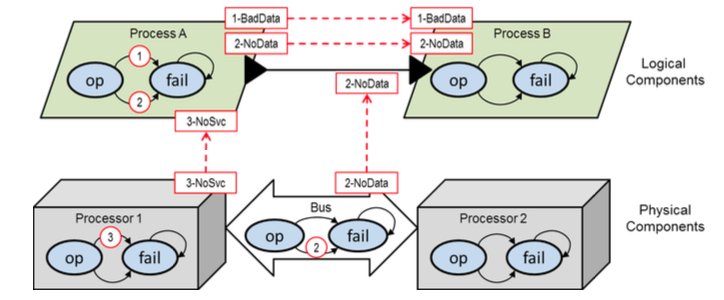
\includegraphics[width=0.9\textwidth]{images/error_annex.png}
  \vspace{-0.1in}
  \caption{Example of Error Model Information and Propagation}
  \label{fig:error_annex}
\end{figure}

An example is shown in Figure~\ref{fig:error_annex}
%\mike{Where is this figure?!?} \danielle{It was in the MBSA section. I have moved it here and if needed will reference from there}.
Errors are labeled with error types: 1-BadData, 2-NoData, 3-NoSvc. Failure events that can cause a component to fail are labeled with the corresponding error number. The error behavior of components is described by their state machines. Note that while all state machines in Figure 2 have two states, they can be much more complex. The dashed arrows indicate propagations describing how failures in one component can cause other components to fail. For example, failures in the physical layer propagate to failures in the associated logical components.

Although the error model annex is very capable, it is not closely tied to the behavioral model of components or their requirements. For example, in the wheel braking system (WBS) example \cite{SAE:ARP4761}, it is possible that hydraulic system valves can fail open or fail closed. In fail closed, downstream components receive no flow and upstream pipes may become highly pressurized as a natural consequence of the failure. Physical models of these behavioral relationships often exist that can propagate failures in terms of the behavioral relationships between components. However, with the AADL error model annex, the propagations must be (re)specified and defined for each component. %The user must therefore model the system twice, specifying propagations in the models of the physical phenomena, and then again using enumerations and propagation rules in state machines in the error model annex.
This re-specification can lead to inconsistencies between physical models and error annex models. In addition, the physical relationships between failures can be complex and may not be describable using enumeration values, leading to additional inconsistencies between the behavior of the physical phenomena and the behavior of the error model.

\iffalse
\danielle{Added from proposal. I believe this describes what you mentioned above, Mike.}
This research attempts to bridge the descriptions of errors in the error model annex with behavioral descriptions of components. We start from the error model notions of error types and state machines that describe transitions from nominal to error states. We then tie these nominal and error states to behavioral models of the components in question. Now these components can provide implicit propagation of the faulty behaviors. The natural consequences of these failures will be manifested in the propagation of other component faults in the behavioral model.

To accomplish this, we use AADL and the error model annex to describe faults and to use the AGREE contract specification language to describe behavioral models. This will require extensions to AGREE to define fault models that describe how different faults manifest themselves in changes to output signals. It will also require changes to the error annex. The conditions under which faults occur will become richer such that they describe not just propagation of enumerations from other components, but also valuations of input signals. For example, very high pressure in a pipe in the WBS model may lead to a \textit{pipe burst} failure.
\fi

\subsection{Failure Effect Modeling (FEM) Approaches}

%\mike{Unfortunately, this is what is done, and done well in xSAP; they have a CAV paper on it; need to account for this}.
%\danielle{I have been trying to find this paper... not sure what it is. I will move on for now and perhaps you have the paper title so that I can add a citation and some accounting for their research.}

In a failure effect modeling approach, the analysis starts from a {\em nominal} model of the system that describes the system behavior when no faults are present.  To perform safety analysis, we then also formalize the fault model. The fault model, in addition to common failure modes such as \emph{non-deterministic}, \emph{inverted}, \emph{stuck\_at} etc, could encode information
regarding fault propagation, simultaneous dependent faults and fault hierarchies, etc.
After specifying the fault model and composing it with the original system model, the safety analysis involves verifying whether the safety requirements hold in presence of the faults defined in the fault model.


%In this work, a behavior fault modeling language was constructed as an extension to the Lustre language \cite{Halbwachs91:IEEE}. Lustre is the kernel language of the popular model-based development tool SCADE \cite{SCADE}.
In this approach, a safety engineer can model different kinds of fault behavior: e.g., stuck-at, ramp-up, ramp-down, and nondeterministic, and then {\em weave} these fault models into the nominal model. The language for describing faults is extensible, allowing engineers to define a catalog of faults appropriate for their domain. In addition, the weaving process allows error propagation between unconnected components within a system model \cite{Joshi07:Hase}. This allows consideration of physical aspects (e.g., proximity of components, shared resources such as power) that may not be present in a logical system model but can lead to dependent failures. In addition, it allows propagation of faults in the reverse direction of the model data flow. This can occur when physical components have coupling such as back-pressure in fluid systems or power surges in the opposite direction of communication through connected components. Finally, it is possible to create fault mediations to describe the output in the presence of multiple simultaneous faults.



%In previous work, component-level modeling tools such as Simulink \cite{MathWorks} and SCADE \cite{SCADE} were extended. In this work, we adapt this process to target system architecture models \cite{AADL, SysML} for safety analysis.

%\subsection{Safety Analysis Approach}

A safety analysis system model can be used for a variety of simulations and analyses.  Modeling allows trivial exploration of \textit{what-if} scenarios involving combinations of faults through simulations.  The current AADL tool suite contains a graphical symbolic simulator that allows for forward and back-stepping through different failure scenarios.  In addition it contains a test-case generator that can automatically generate such scenarios.
For more rigorous analyses, we can use model checking tools to automatically prove (or disprove) whether the system meets specific safety requirements.  As we will demonstrate on the WBS, an engineer first verifies that safety properties hold on the nominal system, an idealized model of the digital controller and the mechanical system containing no faults.  Once the nominal model is shown to satisfy the safety property, the behavior of the fault-extended model can be examined to examine its resilience to faults.

%In our current work, this analysis is performed by determining whether the property held for a given fault threshold: the maximum number of component faults to which the system is expected to be resilient.  This fault threshold is, in some sense, an approximation of the likelihood of component faults. It maps from the probabilistic \textit{real world} potential for component failure into a non-probabilistic verification problem. Recent work in xSAP\cite{CAV2015:BoCiGrMa} uses a more sophisticated approach involving minimum cut sets to describe the set of potential component failures that must be considered; we will likely adopt this approach into our analysis tools.

%Both approaches provide separation between the probabilistic aspects of the real world and the computational demands of formal analysis.


\iffalse
\subsection{Compositional Verification of System Architectures}

As part of the NASA Compositional Verification of Flight Critical Systems (CVFCS) project and the DARPA META and High Assurance Cyber Military Systems (HACMS) projects, we have constructed sophisticated compositional verification tools for reasoning about complex systems architectures. These tools \cite{NFM2012:CoGaMiWhLaLu} allow scaling of formal verification through splitting the analysis of a complex system architecture into a collection of verification tasks that correspond to the structure of the architecture. By decomposing the verification effort into proofs about each subsystem within the architecture, the analysis has been scaled to very large system designs \cite{QFCS15:backes}. In the case of the software for a complex medical drug infusion pump, a monolithic analysis of the design does not terminate in 24 hours, while the compositional approach completes in just over five minutes.
<<<<<<< HEAD
The approach naturally supports an architecture-based notion of requirements refinement based on assume-guarantee contracts. The properties of components necessary to prove a system-level property, including any assumptions about the component environment, in effect define the requirements for those components. The approach allows reuse of the verification that must already be performed on safety-critical software components and enables distributed development by establishing the formal contracts for components that are used to assemble a system architecture. If we are able to establish a system property using only the contracts of its components, we have the means for performing virtual integration of the components. We can use the contract of each component as a specification for suppliers and have a great deal of confidence that if all the suppliers meet their specifications, the integrated system will work properly.
We have implemented this assume-guarantee mechanism for compositional verification as an extension of the AADL language derived from the safety property subset of the property specification language (PSL) \cite{IEEE:PSL}. The Assume-Guarantee Reasoning Environment (AGREE) is our tool for compositional verification of these contracts. Under the CVFCS project, we are currently adding automated bi-directional translation between AGREE contracts and implementation-level properties in languages such as C and Simulink. Initially, we will support translation into MATLAB properties for analysis using the Simulink Design Verifier and C assertions for analysis using source code model checkers (such as CMBC) or test- based verification. Since contracts are abstractions of component implementations, they provide a much more efficient way of representing heterogeneous components in the system model than translating the component models themselves.
=======

The approach naturally supports an architecture-based notion of requirements refinement based on assume-guarantee contracts. The properties of components necessary to prove a system-level property, including any assumptions about the component environment, in effect define the requirements for those components. The approach allows reuse of the verification that must already be performed on safety-critical software components and enables distributed development by establishing the formal contracts for components that are used to assemble a system architecture. If we are able to establish a system property using only the contracts of its components, we have the means for performing virtual integration of the components. We can use the contract of each component as a specification for suppliers and have a great deal of confidence that if all the suppliers meet their specifications, the integrated system will work properly.

We have implemented this assume-guarantee mechanism for compositional verification as an extension of the AADL language derived from the safety property subset of the property specification language (PSL) \cite{IEEE:PSL}. The Assume-Guarantee Reasoning Environment (AGREE) is our tool for compositional verification of these contracts. Under the CVFCS project, we are currently adding automated bi-directional translation between AGREE contracts and implementation-level properties in languages such as C and Simulink. Initially, we will support translation into MATLAB properties for analysis using the Simulink Design Verifier and C assertions for analysis using source code model checkers (such as CMBC) or test- based verification. Since contracts are abstractions of component implementations, they provide a much more efficient way of representing heterogeneous components in the system model than translating the component models themselves.

>>>>>>> 705062d4005b55c503d3e85e228be8e236a1ac1e

\fi



\section{The Safety Annex}
\label{sec:safety_annex}

In this section, we describe the main features and functionality of the Safety Annex. The usage of the terms error, failure, and fault follow their definitions in ARP4754A~\cite{SAE:ARP4754A}. We use {\em fault} as the generic modeling keyword throughout the AADL model hierarchy.

The Safety Annex Users Guide can be found at \url{https://github.com/loonwerks/AMASE/tree/develop} along with the tool plugins and examples described in this technical report. 

\subsection{Modeling Language for System Design}
\label{subsec:aadl-agree}
%Talk about AADL, AGREE, and why safety annex
%Pull AADL/AGREE background from previous papers to support points in the safety process
%Following the motivation/discussion in the process subsection, talk about why we choose to extend AGREE in safety annex, instead of using a separate safety model, or a semi-separate safety model like EMV2.
We are using the Architectural Analysis and Design Language (AADL)~\cite{FeilerModelBasedEngineering2012} to construct system architecture models.  AADL is an SAE International standard~\cite{AADL_Standard} that defines a language and provides a unifying framework for describing the system architecture for ``performance-critical, embedded, real-time systems''~\cite{AADL_Standard}. From its conception, AADL has been designed for the design and construction of avionics systems.  Rather than being merely descriptive, AADL models can be made specific enough to support system-level code generation.  Thus, results from analyses conducted, including the new safety analysis proposed here, correspond to the system that will be built from the model.  

An AADL model describes a system in terms of a hierarchy of components and their interconnections, where each component can either represent a logical entity (e.g., application software functions, data) or a physical entity (e.g., buses, processors). An AADL model can be extended with language annexes to provide a richer set of modeling elements for various system design and analysis needs (e.g., performance-related characteristics, configuration settings, dynamic behaviors). The language definition is sufficiently rigorous to support formal analysis tools that allow for early phase error/fault detection.

The Assume Guarantee Reasoning
Environment (AGREE)~\cite{NFM2012:CoGaMiWhLaLu} is a tool for formal analysis of behaviors in AADL models.  It is implemented as an AADL annex and annotates AADL components with formal behavioral contracts. Each component's contracts can include assumptions and guarantees about the component's inputs and outputs respectively, as well as predicates describing how the state of the component evolves over time.

AGREE translates an AADL model and the behavioral contracts into Lustre~\cite{Halbwachs91:IEEE} and then queries a user-selected
model checker to conduct the back-end analysis. The analysis %is
can be performed compositionally following the architecture hierarchy such that analysis at a higher level is based on the components at the next lower level.  When compared to monolithic analysis (i.e., analysis of the flattened model composed of all components), the compositional approach allows the analysis to scale to much larger systems. 

%In the avionics context, the software functions/applications, the hardware equipment, and the system that is composed of their integration can all be represented as components connected to/composed of/bind to other components in a hierarchical AADL model. AGREE contracts can be used to capture the functional requirements at each level of the hierarchy. Once the model has been reviewed and the requirements captured have been validated, the back-end analysis can be conducted to verify if each level of the model implements its higher level requirements correctly.

%AADL with the AGREE extension serves as a good candidate as the modeling language for describing the system design aspects of a shared system design and safety analysis model. 
In our prior work~\cite{Stewart17:IMBSA}, we added an initial failure effect modeling capability to the AADL/AGREE language and tool set.  We are continuing this work so that our tools and methodology can be used to satisfy system safety objectives of ARP4754A and ARP4761.  

\begin{comment}
In particular, our goals are to:

\begin{itemize}
	\item Provide a comprehensive, qualitative description of the causal relationship between basic failure events and system level safety requirements.
	\item Provide an accurate, quantitative description of the contribution relationship between failure rates of the fault tree basic events and numerical probability requirements at the system level.
\end{itemize}
\end{comment}
%The remainder of the paper describes our approach towards both of the goals.





\subsection{Basic Functionality}

An AADL model of the nominal system behavior specifies the hardware and software components of the system and their interconnections. This nominal model is then annotated with assume-guarantee contracts using the AGREE annex~\cite{NFM2012:CoGaMiWhLaLu} for AADL. The nominal model requirements are verified using compositional verification techniques based on inductive model checking~\cite{2017arXiv171201222G}.

Once the nominal model behavior is defined and verified, the Safety Annex can be used to specify possible faulty behaviors for each component. The faults are defined on each of the relevant components using a customizable library of fault nodes and the faults are assigned a probability of occurrence. A probability threshold is also defined at the system level. This extended model can be analyzed to verify the behavior of the system in the presence of faults. Verification of the nominal model with or without the fault model is controlled through the safety analysis option during AGREE verification.

To illustrate the syntax of the Safety Annex, we use an example based on the Wheel Brake System (WBS) described in ~\cite{AIR6110} and used in our previous work ~\cite{Stewart17:IMBSA}.
The fault library contains commonly used fault node definitions. An example of a fault node is shown below:


\begin{figure*}
	\begin{center}
		%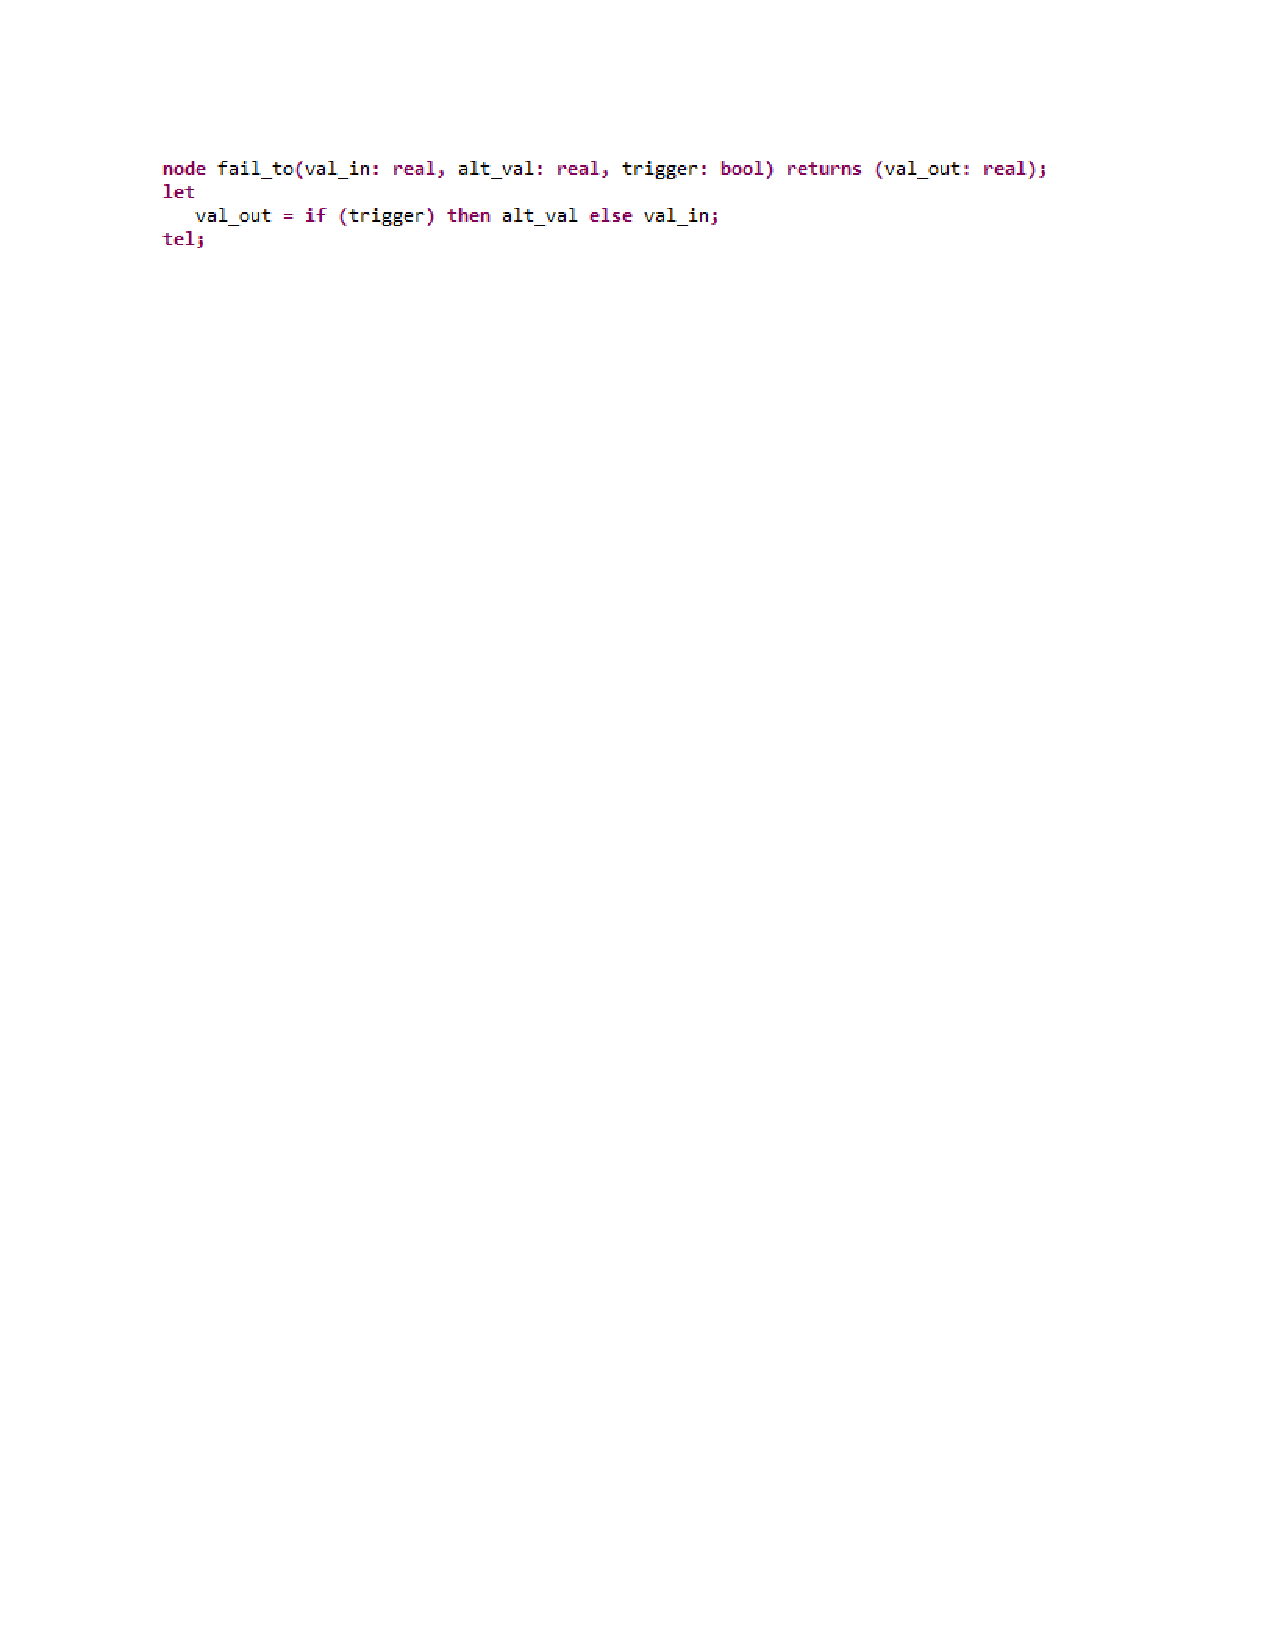
\includegraphics[width=0.6\dimexpr\textwidth-1.5cm\relax]{images/fault_node.pdf}
		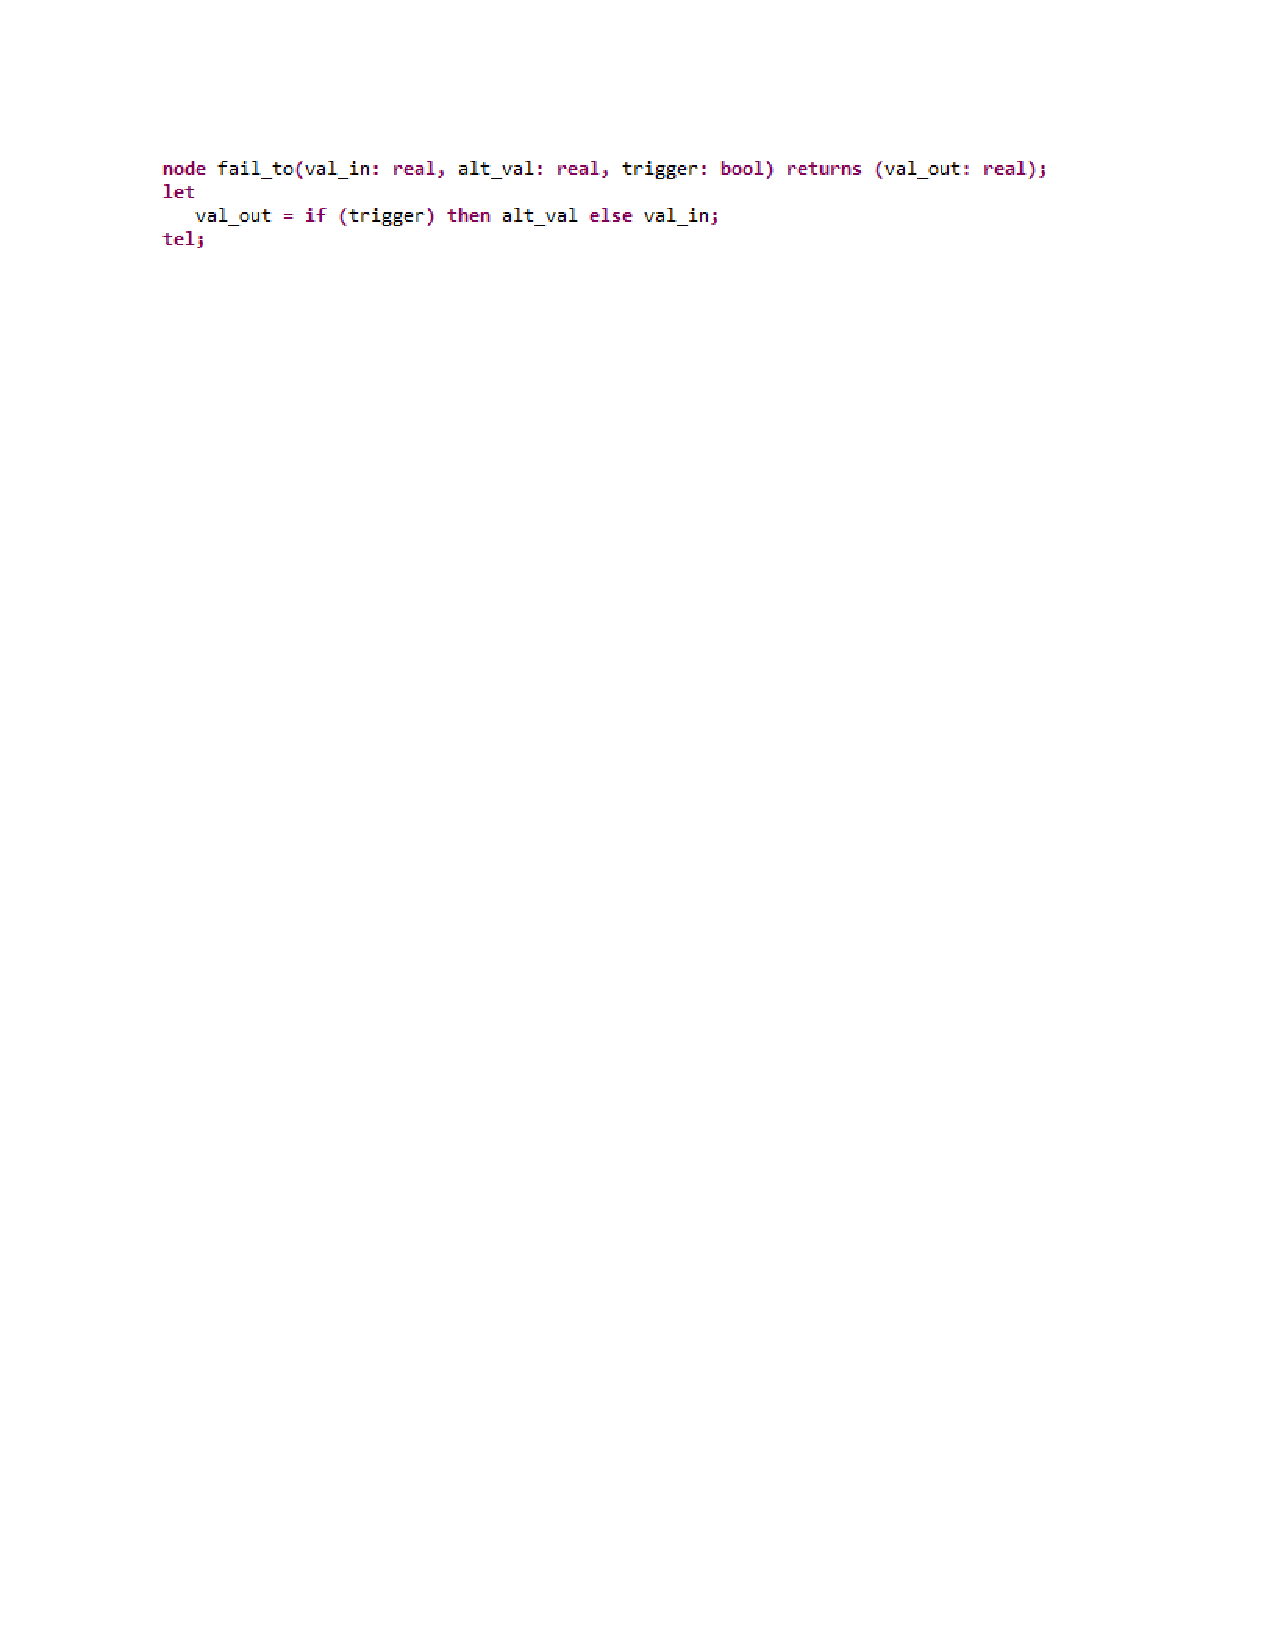
\includegraphics[trim=0 670 -10 70,clip,width=1.3\dimexpr\textwidth-1.5cm\relax]{images/fault_node.pdf}
		\caption{Fault Node Definition in the Safety Annex}
		\label{fig:fault_node}
	\end{center}
\end{figure*}

The \textit{fail\_to} node provides a way to inject a faulty input value. When the \textit{trigger} condition is satisfied, the nominal component output value is overridden by the \textit{fail\_to} failure value. In the WBS, the pump component generates an expected amount of pressure to a hydraulic line.  Declaration of a fail to zero fault in the pump component is shown below:

\begin{figure*}[h!]
	\vspace{-0.6in}
	\begin{center}
		%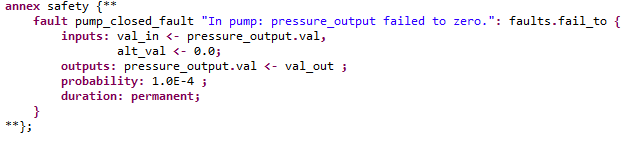
\includegraphics[trim=0 330 150 0,clip,width=1.0\textwidth]{images/pump_fault.png}
		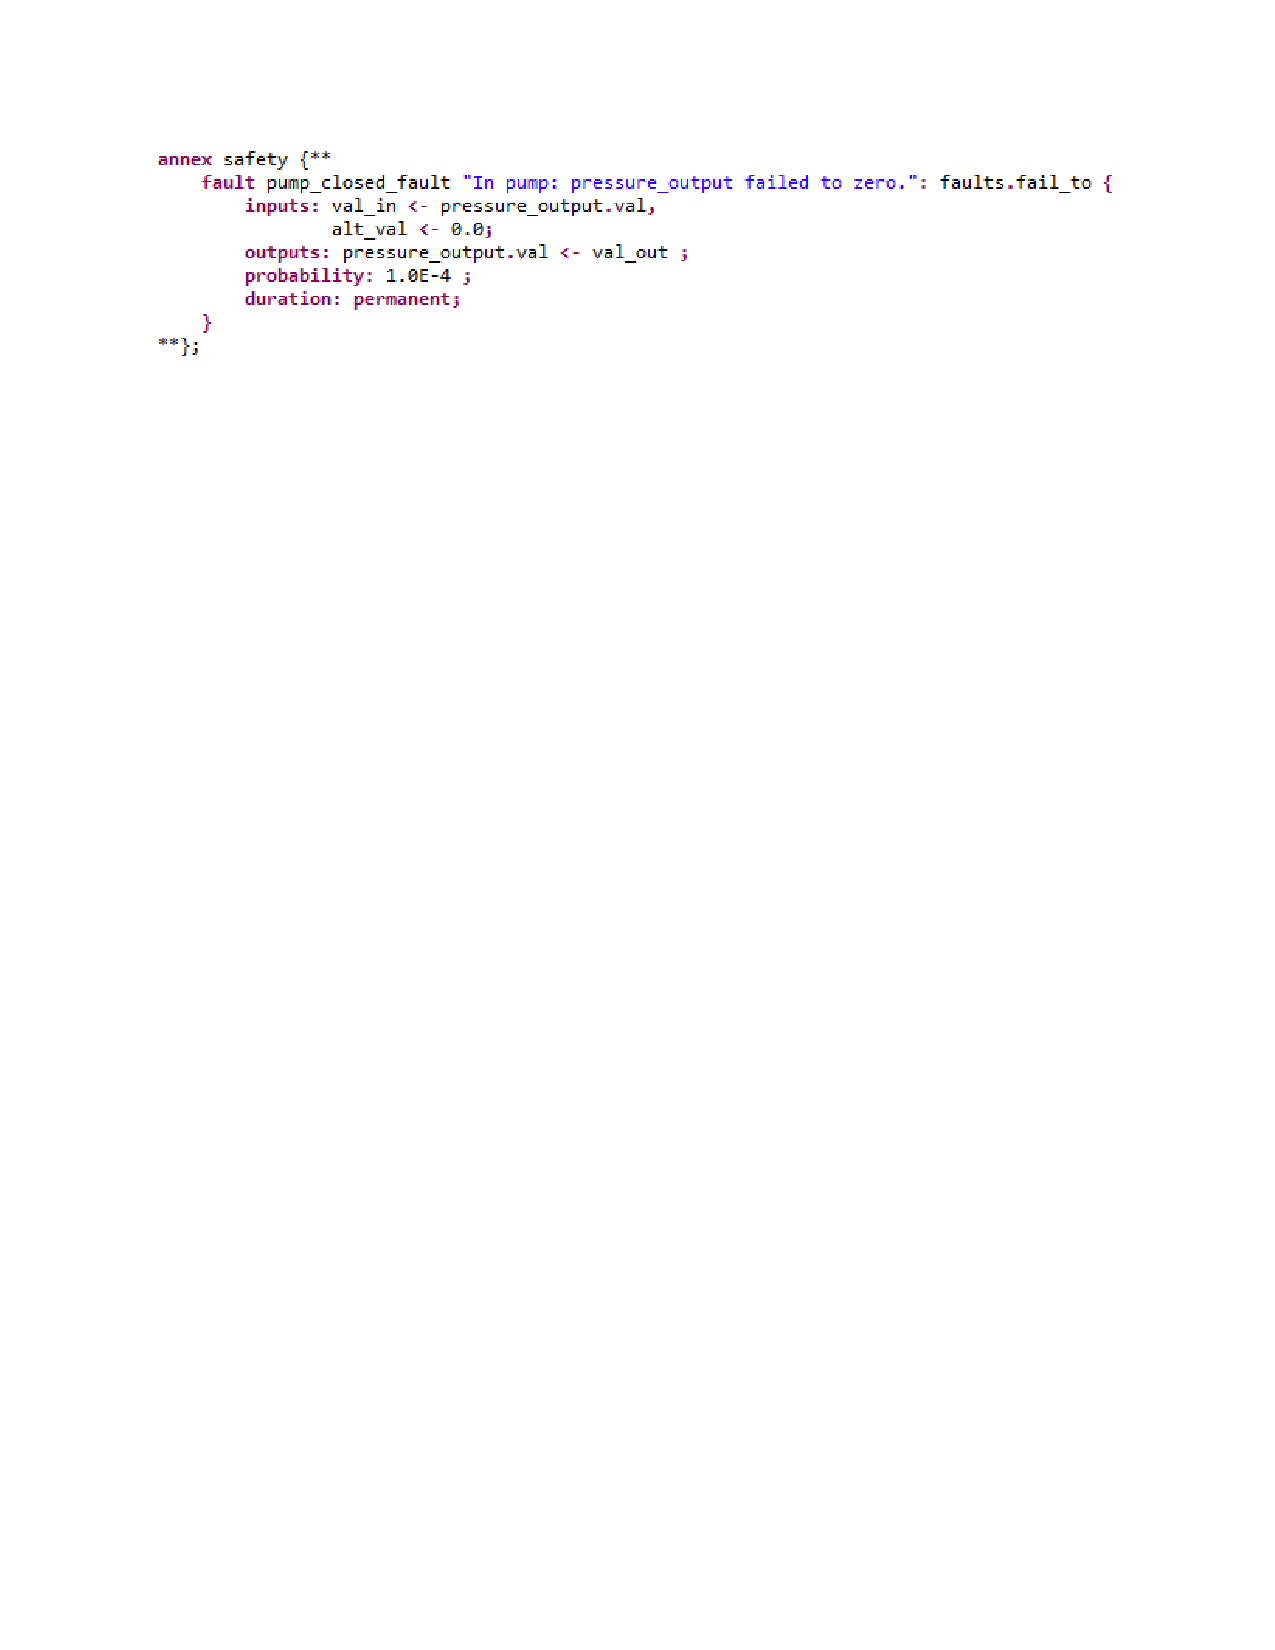
\includegraphics[trim=30 635 0 30,clip,width=1.3\dimexpr\textwidth-1.5cm\relax]{images/pump_fault.pdf}
		\caption{Pump Fault Definition in the Safety Annex}
		\label{fig:fault_node}
	\end{center}
\end{figure*}

The \textit{fault statement} consists of a unique description string, the fault node definition name, and a series of \textit{fault subcomponent} statements. \\
\textbf{Inputs} in a fault statement are the parameters of the fault node definition. In the example above, \textit{val\_in} and \textit{alt\_val} are the two input parameters of the fault node. These are linked to the output from the Pump component (\textit{pressure\_output.val}), and \textit{alt\_value}, a fail to value of zero. When the analysis is run, these values are passed into the fault node definition.\\
\textbf{Outputs} of the fault definition correspond to the outputs of the fault node. The fault output statement links the component output (\textit{pressure\_output.val}) with the fault node output (\textit{val\_out}). If the fault is triggered, the nominal value of \textit{pressure\_output.val} is overridden by the failure value output by the fault node. Faulty outputs can take deterministic or non-deterministic values. \\
\textbf{Probability} (optional) describes the probability of a fault occurrence.\\
\textbf{Duration} describes the duration of the fault; currently the Safety Annex supports permanent faults.\\
%\textit{Equation Statements}: Equation statements support deterministic or nondeterministic types. For more details on equation statements, see ~\cite{NFM2012:CoGaMiWhLaLu}.

\subsection{Hardware Failures and Dependent Faults}

Failures in hardware (HW) components can trigger behavioral faults in the software (SW) or system (SYS) components that depend on them.  For example, a CPU failure may trigger faulty behavior in threads bound to that CPU. In addition, a failure in one HW component may trigger failures in other HW components located nearby, such as cascading failure caused by a fire or water damage.

Faults propagate in AGREE as part of the nominal behavior of a system. This means that any propagation in the HW portion of an AADL model would have to be artificially modeled using data ports and AGREE behaviors in SW. This is less than ideal as there may not be concrete behaviors associated with HW components. In other words, faulty behaviors mainly manifest themselves on the SW/SYS components that depend on the hardware components.

To better model faults at the system level dependent on HW failures, we have introduced a new fault model element for HW components. In comparison to the basic fault statement introduced in the previous section, users are not specifying behavioral effects for the HW failures, nor data ports to apply the failure. An example of a model component fault declaration is shown below:
\begin{figure}[h!]
	\begin{center}
		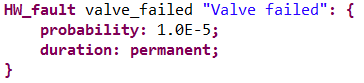
\includegraphics[width=.4\textwidth]{images/hw_fault.png}
		\caption{Hardware Fault in the Safety Annex}
		\label{fig:hardware_fault}
	\end{center}
\end{figure}

In addition, users can specify fault dependencies outside of fault statements, typically in the system implementation where the system configuration that causes the dependencies becomes clear (e.g., binding between SW and HW components, co-location of HW components). This is because fault propagations are typically tied to the way components are connected or bound together; this information may not be available when faults are being specified for individual components. Having fault propagations specified outside of the fault statement of a component also makes it easier to reuse the component in different systems. An example of a fault dependency specification is shown below, showing that the valve{\_}failed fault at the shutoff subcomponent triggers the pressure{\_}fail{\_}blue fault at the selector subcomponent.
\begin{figure*}[h!]
	\begin{center}
		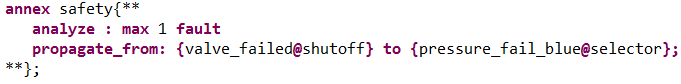
\includegraphics[width=.7\textwidth]{images/fault_propagation.png}
		\caption{Fault Propagation}
		\label{fig:fault_propagation}
	\end{center}
\end{figure*}

\subsection{Architecture and Implementation}

The architecture of the Safety Annex is shown in Figure~\ref{fig:plugin-arch}.  It is written in Java as a plug-in for the OSATE AADL toolset, which is built on Eclipse.  It is not designed as a stand-alone extension of the language, but works with behavioral contracts specified in AGREE AADL annex and associated tools~\cite{NFM2012:CoGaMiWhLaLu}.  AGREE allows {\em assume-guarantee} behavioral contracts to be added to AADL components.  The language used for contract specification is based on the Lustre dataflow language~\cite{Halbwachs91:IEEE}. AGREE improves scalability of formal verification to large systems by decomposing the analysis of a complex system architecture into a collection of smaller verification tasks that correspond to the structure of the architecture.

\begin{figure*}[h!]
	\begin{center}
		%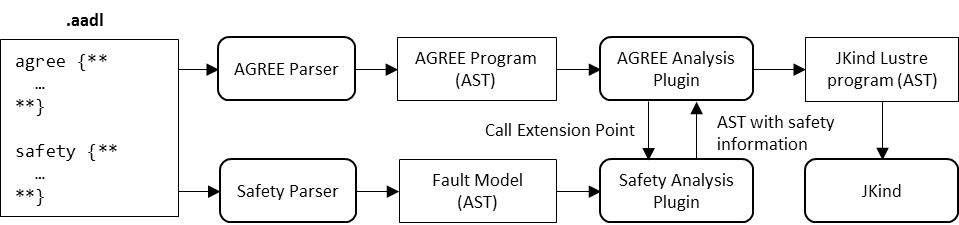
\includegraphics[trim=0 400 430 0,clip,width=0.85\textwidth]{images/arch.png}
		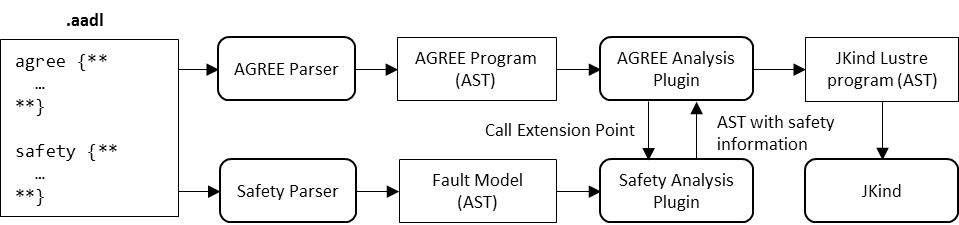
\includegraphics[width=.7\textwidth]{images/arch.png}
	\end{center}
	\caption{Safety Annex Plug-in Architecture}
	\label{fig:plugin-arch}
\end{figure*}

AGREE contracts are used to define the nominal behaviors of system components as {\em guarantees} that hold when {\em assumptions} about the values the component's environment are met.  The Safety Annex extends these contracts to allow faults to modify the behavior of component inputs and outputs.  To support these extensions, AGREE implements an Eclipse extension point interface that allows other plug-ins to modify the generated abstract syntax tree (AST) prior to its submission to the solver.  If the Safety Annex is enabled, these faults are added to the AGREE contract and, when triggered, override the nominal guarantees provided by the component.  An example of a portion of an initial AGREE node and its extended contract is shown in Figure~\ref{fig:comp}.  The \texttt{\_\_fault} variables and declarations are added to allow the contract to override the nominal behavioral constraints (provided by guarantees) on outputs.  In the Lustre language, \texttt{assertion}s are constraints that are assumed to hold in the transition system.

\begin{figure*}[h!]
	%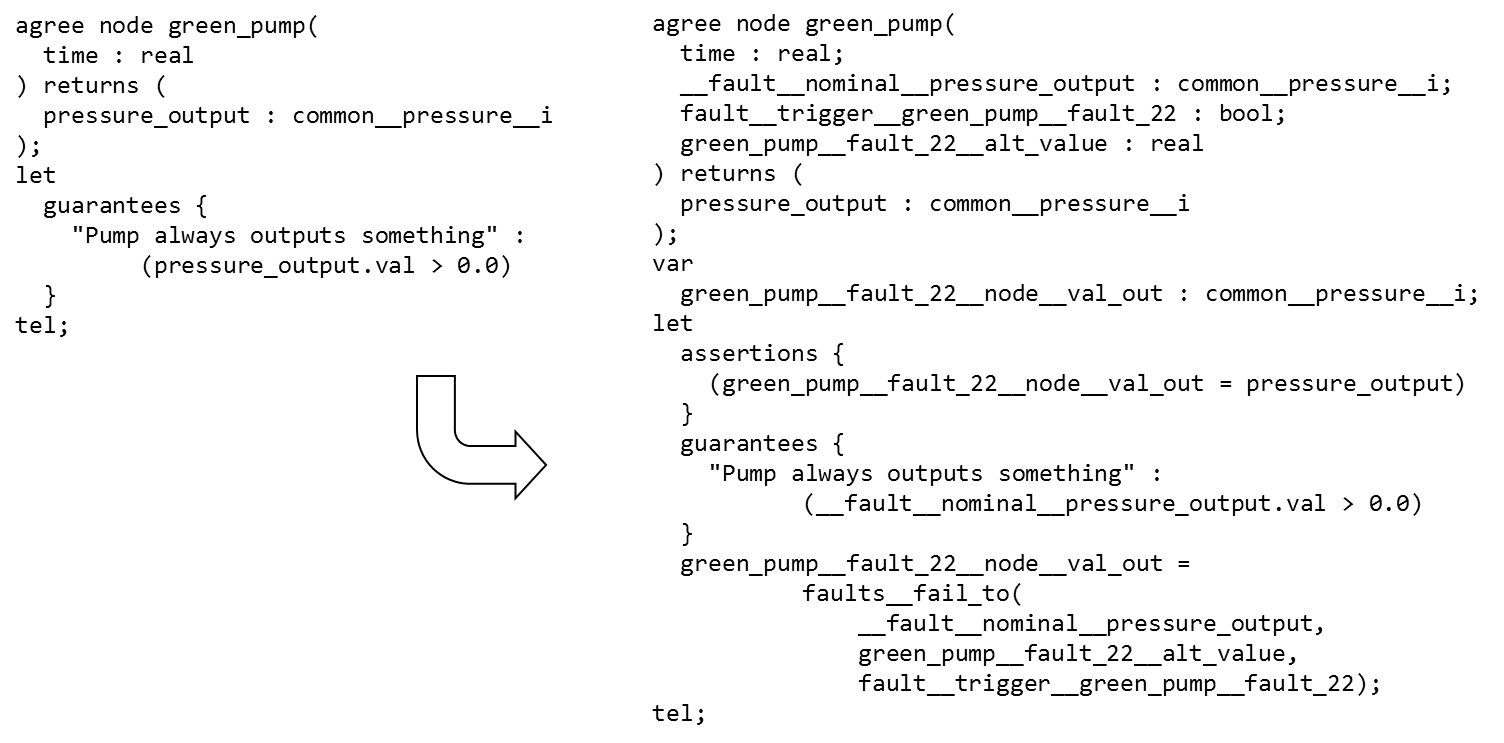
\includegraphics[trim=30 150 120 10,clip,width=\textwidth]{images/sample_code.png}
	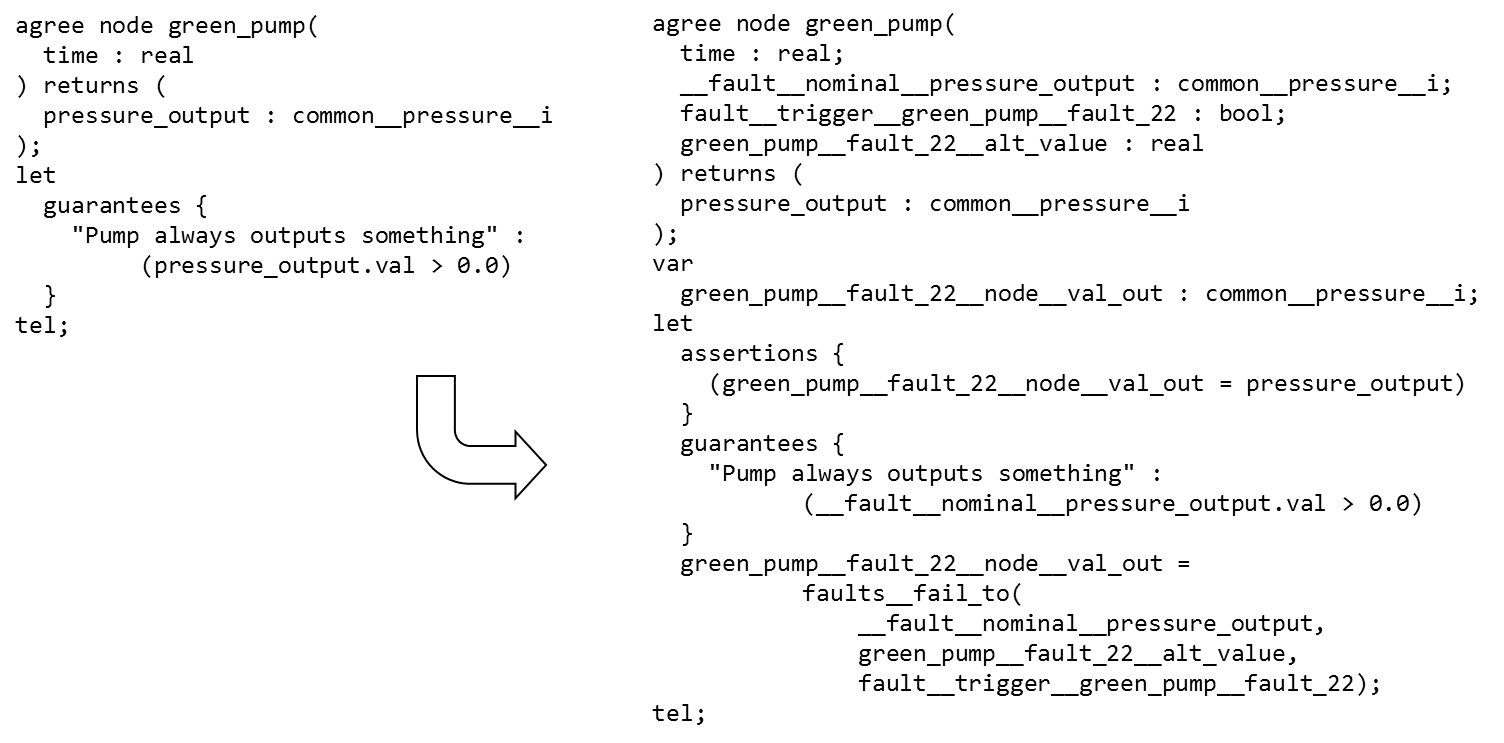
\includegraphics[width=\textwidth]{images/sample_code.png}
	\caption{Nominal AGREE node and its extension with faults}
	\label{fig:comp}
\end{figure*}

An annotation in the AADL model determines the fault hypothesis.  This may specify either a maximum number of faults that can be active at any point in execution (typically one or two), or that only faults whose probability of simultaneous occurrence is above some probability threshold should be considered. In the former case, we assert that the sum of the true {\em fault\_\_trigger} variables is below some integer threshold.  In the latter, we determine all combinations of faults whose probabilities are above the specified probability threshold, and describe this as a proposition over {\em fault\_\_trigger} variables.
%
With the introduction of dependent faults, active faults are divided into two categories: independently active (activated by its own triggering event) and dependently active (activated when the faults they depend on become active). The top level fault hypothesis applies to independently active faults. Faulty behaviors augment nominal behaviors whenever their corresponding faults are active (either independently active or dependently active).

Once augmented with fault information, the AGREE model follows the standard translation path to the model checker JKind~\cite{2017arXiv171201222G}, an infinite-state model checker for safety properties.  The augmentation includes traceability information so that when counterexamples are displayed to users, the active faults for each component are visualized.


%\subsection{Mapping to Safety Analysis Artifacts}

\begin{comment}
The following list describes how the basic safety concepts can be represented using the Safety Annex.

\begin{enumerate}
\item \textbf{Error} Definition and how we model it
\item \textbf{Fault} Definition and how we model it
\item \textbf{Failure} Definition and how we model it. Non deterministic faults
\item \textbf{Failure Mode}
\end{enumerate}


Errors/Faults/Failures - to a safety engineer, these terms have very specific meanings.  You will see my specific comments on this topic where I located them by your Section 3.3.  If needed, we can talk about this comment after I send you my mark-ups.
In Section 3.1, you introduce the term "non-deterministic".  I am not sure how your new process can be used by the safety engineering discipline unless things are "deterministic" and therefore "repeatable".
\end{comment}

\begin{comment}
A prerequisite of performing the safety assessment of a system design is to understand how the system works, primarily focusing on the integrity of the outputs and the availability of the product. The safety engineers then use the acquired understanding to conduct safety analysis, construct the safety analysis artifacts, and compare the analysis results with established safety objectives and safety related requirements.
%check Figure 7 of ARP-4754A for step by step process of the traditional approach
%How our approach can help: step by step process; inputs and outputs
%Drawback/inefficiencies with the current safety assessment
%The causal effect in the fault tree is manually come up by safety engineers after understanding the signal and function flow in the system/sw design documents for the related functionality.
%The logical causal relationship is represented in a descriptive fault tree structure.
%It works well when the signals are processed in a sequential/linear fashion, but not when there are interactions/feedback loops that make the causal effect no longer linear?

%case study
%AIR6110, Rockwell white paper
"working on safety analysis process. Strategy:
1. Check the example Mike Peterson did with stall warning
2. Come up with model in our end
3. See if we can catch anything missed by the fault tree, or help supply the fault tree analysis"
start process investigation by:
1. select the example from stall warning where mike has produced a fault tree from the document
2. independently model from the stall warning doc and try to:
get information from the fault tree that can build the structure of the fault tree
get information from the verification that can help trim/update the probability numbers of the fault tree
3. Compare the fault tree produced by Mike and the information supplied by our study, and see if we provide values to this study
Repeat this for an example fault tree from the white paper Mike sent

Process investigation
How should our model interact with the fault tree that Mike come up with? Any place we can work to create the tree for him? Or provide additional scenarios? Or validate the probabilities for his tree? Or SW/HW/Sys interactions that our approach captures that is hard to capture/verify using his approach?
How does the behavioral/interaction part of the document be modeled in the fault tree and in our model?
What findings from the safety process is driving the model/design updates, such as redundancy?
Would the AMASE modeling and analysis approach justify to make a conservative fault tree less conservative?
How the process steps are different from the process steps for ARP4761A MBSA?

With our process, do we have to use our tool/approach? Or other tools/approaches like xSAP could also work? What's the uniqueness of using our tool in this process? What's the benefit of this process in comparison to the current/traditional safety process?

"Documents to read:
- the white paper by Mike Peterson's group
- ARP4761A model based development supplement
- AIR 6110
- ARP4761
- ARP4754"
According to ARP4761A MBSA supplement draft, the MBSA model is called the Failure Propagation Model (FPM).
ARP4761A MBSA supplement identified some limitation of MBSA, including "it may be difficult to represent complicated Failed Conditions".
Check the simple example (Section 6) in ARP4761A MBSA

Answer from process point of view: why is our approach better than what's out there? What problem are we trying to solve?
Are we doing FPM (Failure Propagation Model) per ARP4761 MBSA?
MBSA section 6.2 shows a complex MBSA example

Give a detailed description of how fault tree is related to the AMASE nominal and faulty model, and the results from the AMASE verificaiton is relayed/fed bak to the fault tree
\end{comment}


 \section{Case Studies}
\label{sec:case_study}
To demonstrate the effectiveness of the Safety Annex, we describe two case studies.



\iffalse
\subsection{Simple Wheel Brake System}
The Wheel Brake System (WBS) described in ARP4761 has been used as a case study for safety analysis, formal verification, and contract based design in numerous studies. In order to show scalability compare results with other tools and studies, the AADL model of the WBS used in~\cite{Stewart17:IMBSA} was enhanced using as a guide the NuSMV ARCH4 model as described in~\cite{DBLP:conf/cav/BozzanoCPJKPRT15}. This version of the WBS model was chosen due to the complexity of the model and because this model addresses required safety concerns (for description of these concerns, see~\cite{DBLP:conf/cav/BozzanoCPJKPRT15}). Due to the added complexity of this WBS system, a short description of the subcomponents and behavior is necessary.

\subsubsection{Simple WBS architecture description}
The highest level model component is the WBS. It consists of the Braking System Control Unit (BSCU), green and blue hydraulic pressure lines (supplied by the green and blue hydraulic pumps respectively), a selector which selects between normal operating mode and alternate operating mode, and the wheel system.

There are three operating modes of the WBS. In \textit{normal} mode, the system uses the \textit{green} hydraulic circuit. In \textit{alternate} mode, the system uses the \textit{blue} hydraulic circuit.  If the BSCU detects lack of pressure from the green line or one of its command units are invalid, then the system switches into alternate mode. The last mode of operation of the WBS is the \textit{emergency} mode. This is supported by the blue circuit but operates if the blue hydraulic pump fails. The accumulator pump has a reserve of pressurized hydraulic fluid and will supply this to the blue circuit in emergency mode.  Antiskid braking commands receive data from the BSCU that will determine if skidding is found at the wheel and handle accordingly.

In the simplified WBS model, there is one wheel that receives pressure from either the green or blue line. This wheel provides feedback to the BSCU providing information about the pressure supplied.

To evaluate the effectiveness of the Safety Annex, we updated the simple WBS model~\cite{Stewart17:IMBSA} to specify faulty component behaviors. The components' nominal  and faulty behaviors are modeled separately. At the top-level AADL component, the fault hypothesis was specified as the maximum number of faults that can be active at any time. The AGREE contracts at the top-level component were verified using AGREE, with the ``Perform Safety Analysis'' option selected. This signals the tool to weave the nominal and faulty behaviors into one augmented AGREE model before feeding to the model checker.

In this example, the top level contract ``Pedal pressed and no skid implies brake pressure applied'' was verified in the presence of at most one fault active during execution.  However, it was shown to be invalid when more than one fault was allowed. The counterexample indicated that both Selector's outputs failed to non-deterministic values due to the faults introduced.
\fi


\subsection{Wheel Brake System}
%original in the case study:
%The Wheel Brake System (WBS) described in ARP4761 has been used as a case study for safety analysis, formal verification, and contract based design in numerous studies. In order to show scalability compare results with other tools and studies, the AADL model of the WBS used in~\cite{Stewart17:IMBSA} was enhanced using as a guide the NuSMV ARCH4 model as described in~\cite{DBLP:conf/cav/BozzanoCPJKPRT15}. This version of the WBS model was chosen due to the complexity of the model and because this model addresses required safety concerns (for description of these concerns, see~\cite{DBLP:conf/cav/BozzanoCPJKPRT15}). Due to the added complexity of this WBS system, we provide a short description of the subcomponents and behavior.
%from related work:
%The Wheel Brake System (WBS) described in ARP4761~\cite{SAE:ARP4761} has been used in the past as a case study for safety analysis, formal verification, and contract based design~\cite{DBLP:conf/cav/BozzanoCPJKPRT15, 10.1007/978-3-319-11936-6-7, CAV2015:BoCiGrMa, Stewart17:IMBSA, propBasedProofSys, Joshi05:SafeComp, NasaRep:MBSA-Aug05} The preliminary work for the safety annex used a simplified model of the WBS~\cite{Stewart17:IMBSA}. In order to show scalability and compare results with other studies, an AADL version of the WBS was designed based off of arch4wbs NuSMV model described in previous work~\cite{DBLP:conf/cav/BozzanoCPJKPRT15}. This model was chosen due to the number of subcomponents in the system and the complexity of behavior captured in the NuSMV model.

The Wheel Brake System (WBS) described in AIR6110~\cite{AIR6110} is a well-known example that has been used as a case study for safety analysis, formal verification, and contract based design~\cite{DBLP:conf/cav/BozzanoCPJKPRT15, 10.1007/978-3-319-11936-6-7, CAV2015:BoCiGrMa, Joshi05:SafeComp}. The preliminary work for the safety annex used a simplified model of the WBS~\cite{Stewart17:IMBSA}. In order to demonstrate scalability of our tools and compare results with other studies, we constructed a functionally and structurally equivalent AADL version of %most complex
one of the most complex WBS xSAP models (arch4wbs) described in 
%previous work
~\cite{DBLP:conf/cav/BozzanoCPJKPRT15}.  %It was chosen due to the complexity of the model and because this model addresses required safety concerns (for description of these concerns, see~\cite{DBLP:conf/cav/BozzanoCPJKPRT15}).
%We describe the elaborations of this model to the ARP4761 WBS below.
%Due to the added complexity of this WBS system, we provide a short description of the subcomponents and behavior.

The Aerospace Information Report 6110 (AIR6110) document provdes an example of a single aircraft system, namely the braking system, for the hypothetical passenger aircraft model S18. The two engine passenger aircraft is designated to carry up to 350 passengers for an average flight time of 5 hours. The purpose of the system is to provide a clear example of systems development and its analysis using the methods and tools described in ARP4754A/ED-79A. This brake system implements the aircraft function \textit{''Decelerate aircraft on the ground (stopping on the runway)"}.  

\subsubsection{WBS overview and architecture description}
The WBS is a hydraulic braking system that provides braking of left and right landing gears, each of which have four wheels. Each landing gear can be individually controlled by the pilot through left/right brake pedals. 

The WBS is composed of two main parts: the control system and the physical system. The control system electronically controls the physical system and contains a redundant Braking System Control Unit (BSCU) in case of failure. In addition to the redundant BSCU channel, the control system is composed of a number of logical components including sensors for the wheels and brake pedal position, a monitor system that checks validity of the BSCU channel, and the command system which commands braking for each of the 8 wheels. The control system is primarily used in the normal mode of operation to command brake pressure.  

The physical system consists of the hydraulic circuits running from hydraulic pumps to wheel brakes. This circuit contains the pumps for both normal and alternate modes of operation (named green and blue lines respectively), a selector valve which selects the circuit depending on input from the BSCU, meter valves at each wheel. These are the physical components that provide braking force to the 8 wheels of the aircraft.

There are three operating modes in the WBS model. In \textit{normal} mode, the system uses the \textit{green} hydraulic circuit. In the normal mode of operation, the selector valve uses the green hydraulic pump to supply fluid to the wheels. Each of the 8 wheels has one meter valve which  are controlled through electronic commands coming from the BSCU. These signals provide brake commands as well as antiskid commands for each of the wheels. The braking command is determined through a sensor on the pilot pedal position. The antiskid command is calculated based on information regarding ground speed, wheel rolling status, and braking commands.

In \textit{alternate} mode, the system uses the \textit{blue} hydraulic circuit.  The wheels are all \textit{mechanically} braked in pairs (one pair per landing gear). The alternate system is composed of the blue hydraulic pump, four meter valves, and four antiskid shutoff valves. The meter valves are mechanically commanded through the pilot pedal corresponding to each landing gear. If the system detects lack of pressure in the green circuit, the selector valve switches to the blue circuit. This can occur if there is a lack of pressure from the green hydraulic pump, if the green hydraulic pump circuit fails, or if pressure is cut off by a shutoff valve. If the BSCU channel becomes invalid, the shutoff valve is closed.

The last mode of operation of the WBS is the \textit{emergency} mode. This is supported by the blue circuit but operates if the blue hydraulic pump fails. The accumulator pump has a reserve of pressurized hydraulic fluid and will supply this to the blue circuit in emergency mode.

The high level wheel brake system architecture is shown in Figure~\ref{fig:wbs1} as shown in AIR6110. 

\begin{figure}[h!]
	\vspace{-0.17in}
	\begin{center}
		%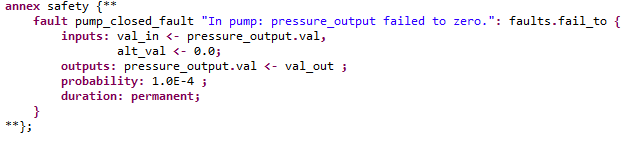
\includegraphics[trim=0 330 150 0,clip,width=1.0\textwidth]{images/pump_fault.png}
		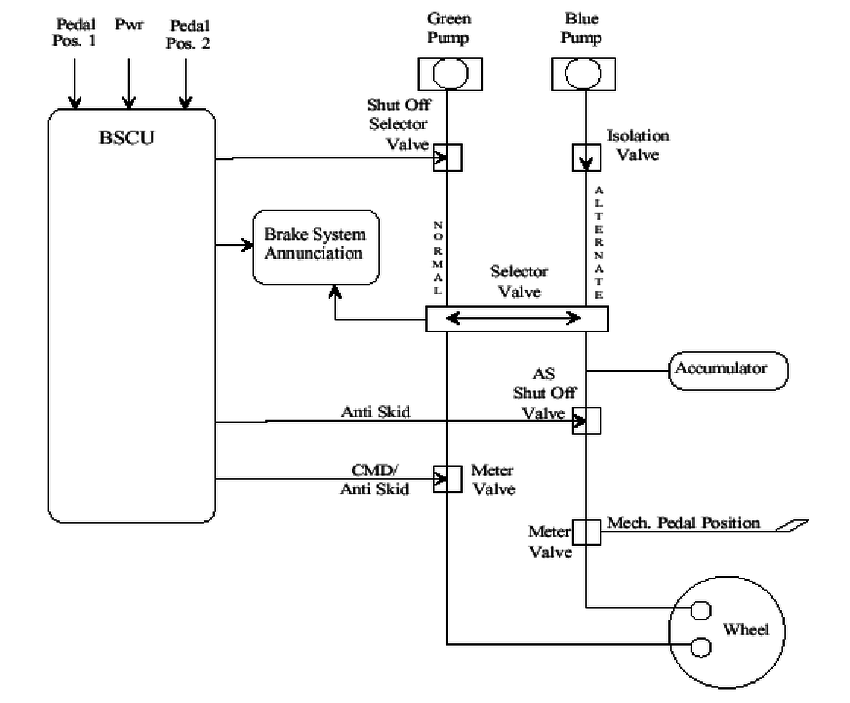
\includegraphics[trim=0 0 0 0,clip,width=1.0\textwidth]{images/wbs_arp4761.png}
		\caption{High level Wheel Brake System}
 		\label{fig:wbs1}
	\end{center}
	\vspace{-0.40in}
\end{figure}

The model contains 30 different kinds of components, 169 component instances, a model depth of 5 hierarchical levels.  The model includes one top-level assumption and  11 top-level system properties, with 113 guarantees allocated to subsystems.  There are a total of 33 different fault types and 141 fault instances within the model.  The large number of fault instances is due to the redundancy in the system design and its replication to control 8 wheels. %\janet{AGREE validates that each component's assumptions are either met by guarantees from another component or system level assumptions. System level assumptions are to be validated manually by system engineers.}

%All assumptions were validated by the AGREE tool (i.e., a component's assumptions are either met by guarantees from another component or assumptions from the top level). %All guarantees were validated by the AGREE tool for the nominal model. Some guarantees for the fault model were invalid (please see the next section for details).

%\mike{An example property would be very useful here!}
An example property is to ensure no inadvertent braking of each of the 8 wheels.  This means that if all power and hydraulic pressure is supplied (i.e., braking is commanded), then either the aircraft is stopped (ground speed is zero), or the mechanical pedal is pressed, or brake force is zero, or the wheel is not rolling.


\subsubsection{Fault Analysis of WBS using Safety Annex}

\iffalse
%After the verification was completed, we defined faults equivalent to those described in the xSAP model for the NuSMV WBS system in~\cite{DBLP:conf/cav/BozzanoCPJKPRT15}.

\begin{figure}[h!]
	\vspace{-0.17in}
	\begin{center}
		%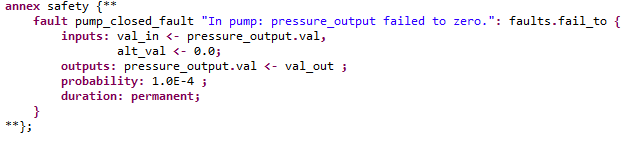
\includegraphics[trim=0 330 150 0,clip,width=1.0\textwidth]{images/pump_fault.png}
		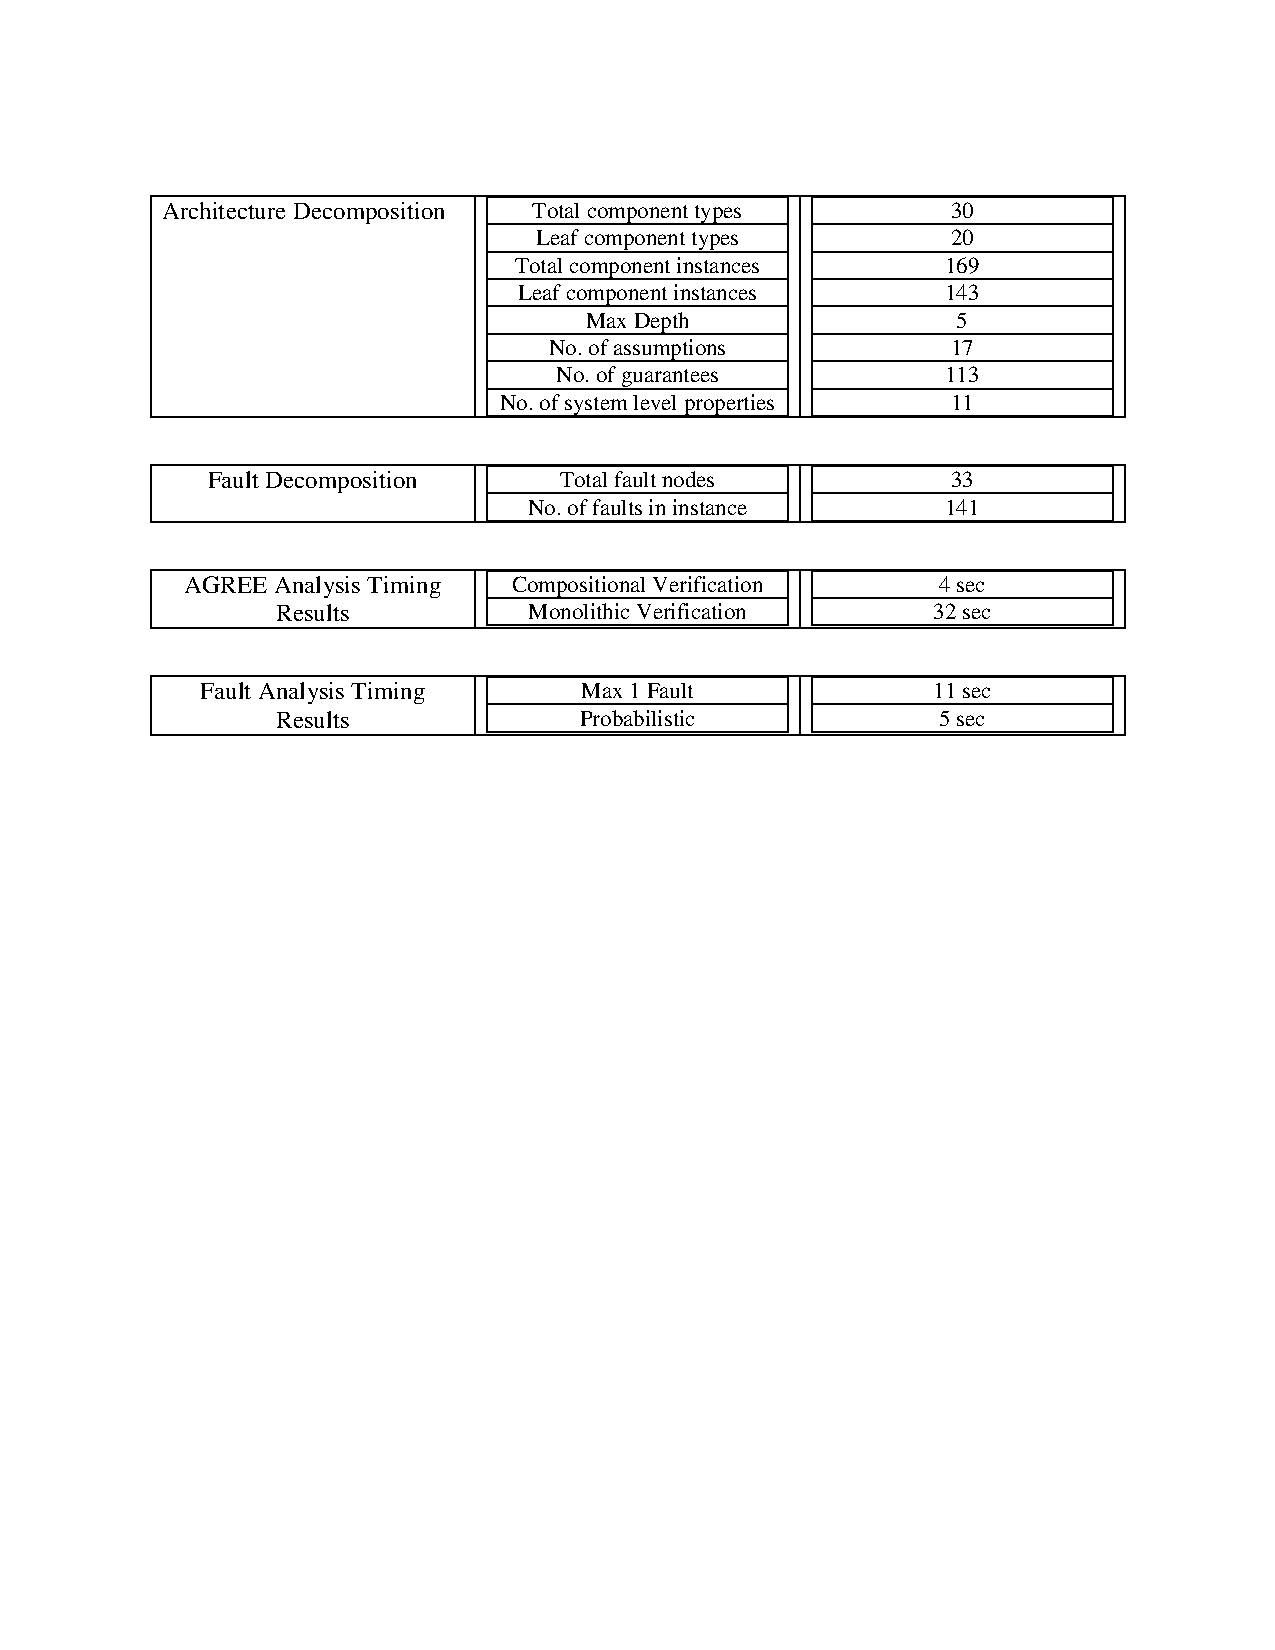
\includegraphics[trim=0 435 0 90,clip,width=1.0\textwidth]{images/arch_table.pdf}
		\caption{Modeling, Verification, and Fault Analysis Metrics}
 		\label{fig:metrics}
	\end{center}
	\vspace{-0.40in}
\end{figure}
\fi


Fault analysis on the top level WBS system was performed on the 11 top-level properties using two fault hypotheses.  In the first case, we allow at most one fault, and in the second we allow combinations of faults that exceed the acceptable probability for the top-level hazard defined in AIR6110.

%original version
%We examine scalability by looking at analysis times for both compositional verification, where the verification task is split into layers to be analyzed separately, and monolithic verification, where the entire system is analyzed in one pass.  When considering the nominal system behavior (no faults), the total time required for analysis using compositional verification is 2 minutes 38 seconds, and the time for monolithic analysis is 30 seconds.  This nominal model is too small to gain significant benefit from compositional analysis.  However, when we consider faulty behavior, when given a single-fault hypothesis, the total time for compositional analysis is 2 minutes 37 seconds, and monolithic analysis did not finish after 42 minutes (ended due to out of memory error), clearly demonstrating the value of compositional analysis for more complex models.  Similarly, for probabilistic analysis, the compositional time is 2 minutes 38 seconds and the monolithic time is 3 minutes 31 seconds.

%first updated version
%We examine scalability by looking at analysis times for both compositional verification, where the verification task is split into layers to be analyzed separately, and monolithic verification, where the entire system is analyzed in one pass.  When considering the nominal system behavior (no faults), the total time required for analysis using compositional verification is 2 minutes 5 seconds, and the time for monolithic analysis is 26 seconds.  This nominal model is too small to gain significant benefit from compositional analysis.  However, when we consider faulty behavior, when given a single-fault hypothesis, the total time for compositional analysis is 2 minutes 6 seconds, and monolithic analysis was not able to determine all results after 3 minutes 35 seconds (ended due to out of memory error), clearly demonstrating the value of compositional analysis for more complex models.  Similarly, for probabilistic analysis, the compositional time is 2 minutes 6 seconds and the monolithic time is 4 minutes. Note that for probabilistic analysis, we use compositional analysis to examine counterexamples for invalid properties, but rely on monolithic analysis to confirm valid properties, as the tool support for aggregated probabilities in compositional setting has not yet been implemented.

We use this model to demonstrate the benefits of formal fault analysis and to show the scalability of our tools.  We applied both {\em monolithic} analysis, in which the entire model is flattened and analyzed at once, and also {\em compositional} analysis, where each architectural layer is analyzed hierarchically.
For the fault-free ``nominal'' system model, monolithic analysis requires 21 seconds, whereas compositional analysis requires 1 minute and 53 seconds.  Although the compositional time is longer, each sub-problem completes in less than 5 seconds.  The additional time for compositional analysis is  due to the start-up overhead to invoke the JKind model checker many times for individual layers.  On the other hand, when examining the model under a single-fault hypothesis, compositional analysis requires 2 minutes 6 seconds, while monolithic analysis did not terminate after 60 minutes.

For probabilistic fault hypotheses, we are currently developing a sound approach for composition with respect to the top-level fault probability, but our current tool requires monolithic analysis.  In this case, given a probabilistic fault hypothesis of $5*10^{-7}$, monolithic analysis requires 3 minutes 25 seconds.

During our analysis, we discovered that most properties were verified, but the \textit{Inadvertent braking at the wheel} properties are not resilient to a single fault nor do they meet the desired $10^{-9}$ fault threshold for probabilistic analysis.  In our model (as in the NuSMV model~\cite{DBLP:conf/cav/BozzanoCPJKPRT15}), there is a single pedal position sensor for the brake pedal.  If this sensor fails, it can command braking without a pilot request.  Given the {\em counterexample} returned by the tools, it is straightforward to diagnose the fault conditions that lead to property failure.

This counterexample can be used to further analyze the system design.  For our model, there are several possible reasons for failure: it could be that that redundant sensors are required on the pedals (here we note that the architecture of the pedal assembly is not discussed in AIR6110), or that the phase of flight is sufficiently short that we need to adjust our pedal failure rate to match this phase of flight, rather than normalizing the failure rate to per-flight-hour.  It is straightforward and computationally inexpensive to run the analysis, allowing quick iterations between systems and safety engineers. As indicated in Figure~\ref{fig:interaction_with_FTA}, the sync and update between the preliminary system FTA and the architecture/analysis model continues until the system safety property is satisfied with the desired fault tolerance and failure probability achieved.

%In terms of the safety analysis process, this corresponds with an update in the preliminary system FTA which will eventually change the system FTA and impact SSA results.\mike{keep last sentence?}

%Mike: with regard to the safety process sentence at the end of the WBS case study, he thinks that we can keep that sentence, but update it to mention that we can iteratively run analysis if we don't achieve the desired fault tolerance for single failure or achieve the desired probability


\subsection{Quad-Redundant Flight Control System}
We have also used the Safety Annex to examine more complex fault types, such as asymmetric (or {\em Byzantine}) faults.  A Byzantine fault presents different symptoms to different observers, so that they may disagree regarding whether a fault is present.
We extended the Quad-Redundant Flight Control System (QFCS) example~\cite{QFCS15:backes} to model and analyze various types of faulty behaviors. Faulty behaviors were introduced to analyze the response of the system to multiple faults, and to evaluate fault mitigation logic in the model. As expected, the QFCS system-level properties failed when unhandled faulty behaviors were introduced.

We also used the Safety Annex to explore more complicated faults at the system level on a simplified QFCS model with cross-channel communication between its Flight Control Computers.

\begin{itemize}
	\item Byzantine faults~\cite{Driscoll-Byzantine-Fault} were simulated by creating one-to-one connections from the source to multiple observers so that disagreements could be introduced by injecting faults on individual outputs. The system level property ``at most one flight control computer in command'' was falsified in one second in the presence of Byzantine faults on the baseline model. The same property was verified in three seconds on an extended model with a Byzantine fault handling protocol added.  System designers can use this approach to verify if a system design is resilient to Byzantine faults, examine vulnerabilities, and determine if a mitigation mechanism works.

%original wording:	
	% A system-level property failed due to the fault on the baseline model, but did not fail on the model with Byzantine fault handling protocol added. Using the Safety Annex like this can test a system's vulnerability to Byzantine faults and verify mitigation mechanisms.
	
	\item Dependent faults were modeled by first injecting failures to the cross-channel data link (CCDL) bus (physical layer), and faults to the flight control computer (FCC) outputs (logical layer), then specifying fault propagations in the top level system implementation (where the data connections between FCC outputs were bound to the CCDL bus subcomponents). The fault propagation indicates that one CCDL bus failure can trigger all FCC output faults. With the fault hypothesis that allows a maximum of one fault active during execution, the system level property ``not all FCCs fail at the same time'' was falsified in one second.
	
%original wording:
%Dependent faults were modeled by injecting failures to hardware components (physical layer), and faults to software components (logical layer) that are bound to the hardware components, then specifying fault propagations at the QFCS system level to indicate that the software faults are dependent on the hardware failures. 	
\end{itemize}

%\mike{Results?} \janet{updated the last two paragraphs}


\section{Future Work}
\label{sec:future_work}

%Address NFM review comments

Formal model based systems engineering (MBSE) methods and tools now permit system level requirements to be specified and analyzed early in the development process~\cite{QFCS15:backes,CIMATTI2015333, NFM2012:CoGaMiWhLaLu, hilt2013:MuWhRaHe}. Design models from which aircraft systems are developed can be integrated into the safety analysis process to help guarantee accurate and consistent results. There are tools that currently support reasoning about faults in architecture description languages such as SysML and AADL. These tools include the AADL Error Model Annex, Version 2 (EMV2)~\cite{EMV2} and HiP-HOPS for EAST-ADL~\cite{CHEN201391}. These approaches primarily utilize \textit{qualitative} reasoning. Faults are enumerated and the propagations through system components are explicitly described. Given many possible faults, these propagation relationships increase in complexity and understandability. Interactions are easily overlooked by analysts and thus not explicitly described. This is also the case with tools like SAML that incorporate both \textit{qualitative} and \textit{quantitative} reasoning~\cite{Gudemann:2010:FQQ:1909626.1909813}.  


%original version:
%In earlier work, an approach to MBSA was demonstrated using the Simulink notation~\cite{Joshi05:SafeComp,Joshi05:Dasc,NasaRep:MBSA-Aug05} . In this approach, a behavioral model of system dynamics was used to reason about the effects of faults in the system. We believe this approach allows an implicit and natural notion of fault propagation through the system. Since Simulink is not an architecture description language, notions such as hardware devices and non-functional aspects cannot be captured in system models. Using this idea of \textit{quantitative} reasoning and implicit fault propagation, we wish to apply this to a more rich architecture language.

%updated version:
%<<<<<<< HEAD
In earlier work, an approach to MBSA was demonstrated using the Simulink\textsuperscript{\textregistered} notation~\cite{Joshi05:SafeComp,Joshi05:Dasc}. In this approach, a behavioral model of system dynamics was used to reason about the effects of faults in the system. This approach allows an implicit and natural notion of fault propagation through the system. However, non-functional architectural properties were not captured as Simulink is not designed as an architecture description language. In our approach, we are applying \textit{quantitative} reasoning and implicit fault propagation to a more rich architecture language.  

There are other tools purpose-built for safety analysis, including AltaRica~\cite{PROSVIRNOVA2013127}, smartIFlow~\cite{info8010007} and xSAP~\cite{DBLP:conf/tacas/BittnerBCCGGMMZ16}. These notations are separate from the system development model, but allow similar behavioral analysis to our tools.  Integration of MBSA into safety analysis process is described by Bozzano and Villafiorita~\cite{Bozzano:2010:DSA:1951720}.
%=======
%In earlier work, an approach to MBSA was demonstrated using the Simulink\textsuperscript{\textregistered} notation~\cite{Joshi05:SafeComp,Joshi05:Dasc,NasaRep:MBSA-Aug05}. In this approach, a behavioral model of system dynamics was used to reason about the effects of faults in the system. This approach allows an implicit and natural notion of fault propagation through the system. However, non-functional architectural properties were not captured as Simulink is not designed as an architecture description language. In our approach, we are applying \textit{quantitative} reasoning and implicit fault propagation to a more rich architecture language.
%>>>>>>> 80fb5bd8b3b71f60ab4a407a2ee73f016effe2c2

Formal verification tools based on model checking have been used to automate the generation of safety artifacts% and used in safety critical system certification
~\cite{symbAltaRica,10.1007/978-3-540-75596-8-13, DBLP:conf/tacas/BittnerBCCGGMMZ16}. This approach has limitations in terms of scalability and readability of the fault trees generated. Work has been done towards mitigating these limitations by the scalable generation of readable fault trees~\cite{10.1007/978-3-319-11936-6-7}.

%Moved the following to case study
%The Wheel Brake System (WBS) described in ARP4761~\cite{SAE:ARP4761} has been used in the past as a case study for safety analysis, formal verification, and contract based design~\cite{DBLP:conf/cav/BozzanoCPJKPRT15, 10.1007/978-3-319-11936-6-7, CAV2015:BoCiGrMa, Stewart17:IMBSA, propBasedProofSys, Joshi05:SafeComp, NasaRep:MBSA-Aug05} The preliminary work for the safety annex used a simplified model of the WBS~\cite{Stewart17:IMBSA}. In order to show scalability and compare results with other studies, an AADL version of the WBS was designed based off of arch4wbs NuSMV model described in previous work~\cite{DBLP:conf/cav/BozzanoCPJKPRT15}. This model was chosen due to the number of subcomponents in the system and the complexity of behavior captured in the NuSMV model.



\section{Conclusion}

We have developed an extension to the AADL language with tool support for formal analysis of system safety properties in the presence of faults. Faulty behavior is specified as an extension of the nominal model, allowing safety analysis and system implementation to be driven from a single common model. This new Safety Annex leverages the AADL structural model and nominal behavioral specification (using the AGREE annex) to propagate faulty component behaviors without the need to add separate propagation specifications to the model.   Next steps will include extensions to automate injection of Byzantine faults as well as automatic generation of fault trees.  For more details on the tool, models, and approach, see the technical report~\cite{SATechReport}.

\vspace{2 mm}
\noindent {\bf Acknowledgments.} This research was funded by NASA contract NNL16AB07T and the University of Minnesota College of Science and Engineering Graduate Fellowship.




\bibliographystyle{abbrv}
\bibliography{biblio}
%\vspace{-7.25cm}
% This ~ seems to fix an odd bibliography alignment issue
~

%\ifdefined\TECHREPORT
%\appendix
%
%\section{Appendix: Proof of Equivalence}
%\input{appendix}
%\fi

%\section{Appendix: GPCA CENTA Model}
%\label{appendix:gpcacenta}
%\begin{figure}[!ht]
%\begin{center}
%\includegraphics[scale=0.6]{images/sampled_pca.PNG} %[trim = 0 2 0 0, clip=true]{Comp}
%\caption{GPCA AGREE Properties modeled as a Timed Automata} \label{fig:samplepca}
%\end{center}
%\end{figure}

%\balancecolumns

\end{document} 